\documentclass[11pt]{article} % 11-pt font size
\usepackage{titling}
\usepackage[left=1in, right=1in, top=1in, bottom=1in]{geometry}  % Set 1-inch margins
\usepackage{multicol} % Include the multicol package
\usepackage{graphicx} % Required for inserting images
\usepackage{enumitem} % Cleaner package for numbering 
% \usepackage[style=apa, backend=biber]{biblatex} % Package for references APA
\usepackage{hyperref} % For clickable links
\usepackage[english]{babel}
\usepackage[utf8x]{inputenc}
\usepackage{amsmath}
\usepackage{graphicx}
\graphicspath{{Images/}}
\usepackage{float}
\usepackage[colorinlistoftodos]{todonotes}
\usepackage{booktabs}
\usepackage{subcaption}
\usepackage{listings}
\usepackage{hyperref}
\usepackage{tabularray}
\begin{document}
    \begin{titlepage}
    
    \newcommand{\HRule}{\rule{\linewidth}{0.5mm}} % Defines a new command for the horizontal lines, change thickness here
    
    \center % Center everything on the page
    %----------------------------------------------------------------------------------------
    %	HEADING SECTIONS
    %----------------------------------------------------------------------------------------
    
    \textsc{\LARGE Georgia Institute of Technology}\\[1.5cm] % Name of your university/college
    \includegraphics[scale=.6]{images/GeorgiaTech_RGB.png}\\[1cm] % Include a department/university logo - this will require the graphicx package
    
    %----------------------------------------------------------------------------------------
    %	TITLE SECTION
    %----------------------------------------------------------------------------------------
    
    \HRule \\[0.4cm]
    { \huge \bfseries Amazon Product Bundling\\\&\\Recommendation}\\[0.4cm] % Title of your document
    \HRule \\[1.5cm]
    
    \textsc{\Large ISYE 7406 -  Data Mining and Statistical Learning}\\[0.5cm]
    \textsc{\large 7406 Project Group 115}\\[0.6cm]
    {\large \today}\\[2cm]
    \begin{center}
    \begin{minipage}{0.33\textwidth}
        \centering
        {\Large Ashish Puri} \\
        apuri61@gatech.edu \\
        GTID:903753582
    \end{minipage}%
    \begin{minipage}{0.33\textwidth}
        \centering
        {\Large Jagannath Banerjee} \\
        jbanerjee7@gatech.edu \\
        GTID:903860232
    \end{minipage}
    \begin{minipage}{0.33\textwidth}
        \centering
        {\Large Piyush Shivrain} \\
        pshivrain3@gatech.edu \\
        GTID:903762723
    \end{minipage}
    \end{center}
\end{titlepage}

\section{Abstract}
Product bundling and customer recommendation are vital strategies in modern marketing practices aimed at enhancing customer satisfaction and increasing sales. According to Zendesk\cite{7}, 62\% of consumers agree that personalized recommendations are better than general ones.According to Porch Group Media \cite{8}, 86\% of consumers say personalization plays a role in their purchasing decisions and 45\% of online shoppers are more likely to shop on a site that offers personalized recommendations.

Product bundling and customer recommendation mechanisms are integral components of Amazon's sophisticated marketing and sales strategies. This paper investigates the intricate interplay between product bundling and customer recommendation systems within the context of Amazon's e-commerce sales data from 2011 to 2014. It examines how Amazon leverages product bundling to offer customers curated bundles of complementary or related items, enhancing the value proposition and driving incremental sales. Additionally, the paper explores customer recommendation algorithms, which analyze user data to deliver personalized product suggestions tailored to individual preferences and purchasing behaviors thereby driving customer engagement, satisfaction, and loyalty on the platform and enhancing the overall customer experience in the digital marketplace.
\section{Introduction}
The objective of this project is to conduct a comprehensive analysis of Amazon sales data to gain valuable insights into sales trends, customer purchase behavior, and other factors influencing profitability. Leveraging various data mining techniques such as exploratory data analysis, clustering, association mining, and predictive modeling, we aim to extract meaningful patterns and relationships to build a product bundling strategy and recommend focused products to customers. By delving into multifaceted dimensions such as product categories, geographical distributions, and sales performance metrics, this analysis will furnish actionable insights to refine sales strategies and augment overall profitability.
\section{Literature Survey}
Currently, customer recommendation is accomplished through a combination of traditional and advanced techniques which includes text mining with qualitative reviews and quantitative ratings \cite{9}\cite{10} and content-based recommender systems, collaborative recommender systems and hybrid recommender systems\cite{11}.We realized collaborative filtering methodology to be the most efficient way to perform customer recommendation system.We implemented the collaborative filtering thoery explained in this paper.Collaborative approaches\cite{11} make use of the measure of similarity between users. This technique starts with finding a group or collection of user X whose preferences, likes, and dislikes are similar to that of user A. X is called the neighbourhood of A. The new items which are liked by most of the users in X are then recommended to user A. The efficiency of a collaborative algorithm depends on how accurately the algorithm can find the neighbourhood of the target user. 
\section{Data Source \& High level understanding}
In order to implement Collaborative Filtering for customer recommendation, we used Amazon sales dataset\cite{1}, downloaded from \href{https://www.kaggle.com/datasets/anandshaw2001/amazon-sales-dataset}{Kaggle}.Data contains order information from 2011 to 2014.It consists of 3204 rows and 9 columns. Following are the attributes in the dataset: 
% Please add the following required packages to your document preamble:
% \usepackage{booktabs}
\begin{table}[H]
\centering
\begin{tabular}{@{}ll@{}}
\toprule
\textbf{Column Name} & \textbf{Column Description}                          \\ \midrule
Order Date           & Order Request Date                                   \\
Ship Date            & Shipping Date                                        \\
Email ID             & Email ID of Users                                    \\
Geography            & Location of Orders by Users                          \\
Category             & Product Category                                     \\
Product Name         & Product Name of Amazon                               \\
Sales                & Amazon Product Sales                                 \\
Quantity             & How many units of a particular product are available \\
Profit               & Amazon Sales Profit                                  \\ \bottomrule
\end{tabular}
\end{table}
We analyzed the sales trend spanning 2011 to 2014, both in its raw form and adjusted for inflation at a rate of 6\%. Our findings revealed a 10 fold surge in sales from 2011 to 2015. We also understood our sales data contains information from west coast of United States.Additionally, we looked at the profitable product, assuming to be important for recommendation. Overall, this tremendous sales growth underscores the significance of strategic customer recommendations through targeted initiatives for up selling and cross-selling.
\begin{figure}[H]
    \centering
    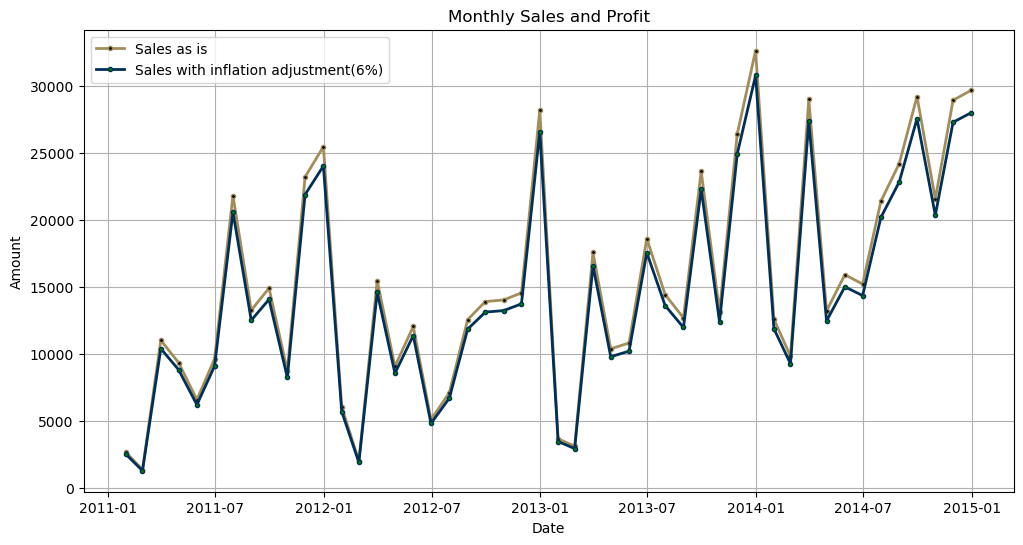
\includegraphics[scale=0.4]{images/sales_inflation_adjustment.png}
    \caption{Sales growth year over year regular and inflation adjusted.}
    \label{fig:Sales growth}
\end{figure}

\begin{figure}[H]
  \centering
  \begin{subfigure}[b]{0.4\textwidth}
    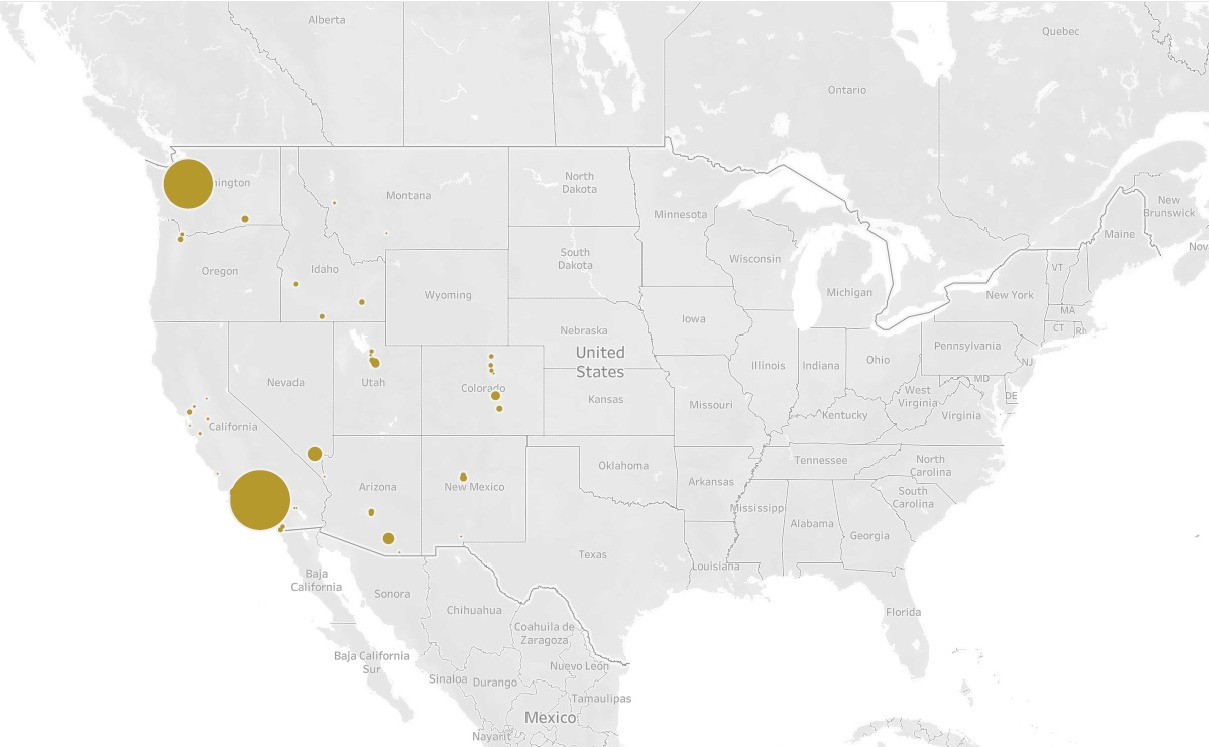
\includegraphics[width=\textwidth]{images/EDA_Geography.jpg}
    \caption{Overall Sales by States in United States}
    \label{fig:sub1}
  \end{subfigure}
  \hfill
  \begin{subfigure}[b]{0.4\textwidth}
    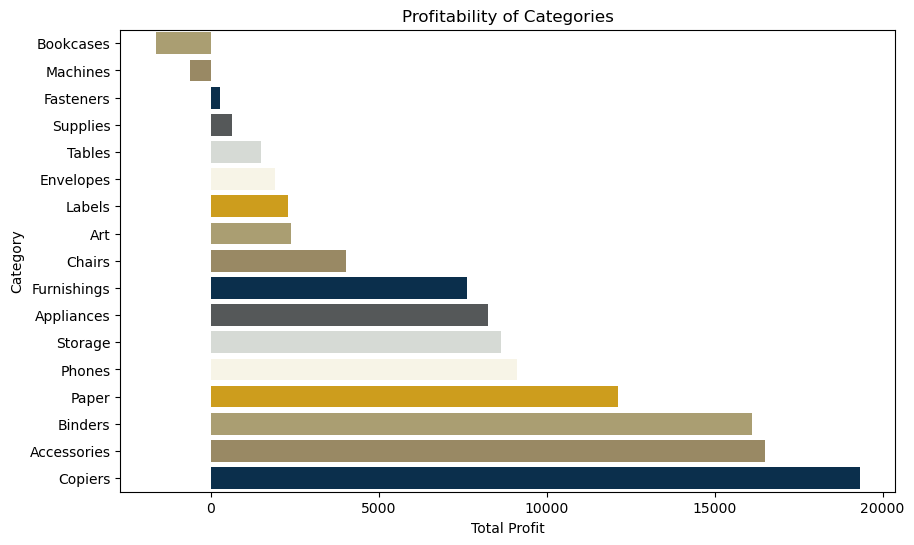
\includegraphics[width=\textwidth]{images/EDA_profitable_category.png}
    \caption{Profitable Product Categories}
    \label{fig:sub2}
  \end{subfigure}
  \caption{Sales by Geography \& Profitable Products}
  \label{fig:twosidebyside}
\end{figure}


\section{Research Questions}
While implementing this paper for project, we aim to investigate fundamental research inquiries aimed at analyzing Amazon sales and find avenues for up-sell and cross-sell recommendation strategies. Specifically, our study seeks to address the following questions: 
\begin{itemize}
    \item Which products possess bundling potential to facilitate up-sell and cross-sell opportunities?
    \item What criteria can be employed to identify customers suitable for bundled product recommendations?
    \item Is it feasible to delineate customer segments conducive to bulk recommendations?
    \item What magnitude of revenue growth can be expected from the implementation of these recommendation strategies
\end{itemize}
By delving into these research questions, we aims to provide valuable insights into Amazon's sales ecosystem and identify actionable strategies to enhance revenue generation and customer satisfaction.


\section{Proposed Methodology}

To analyze Amazon sales data and create a recommendation system we employed a combination of  advanced data mining techniques like clustering, association rule mining and collaborative filtering to understand the product grouping and customer buying patterns.

\subsection*{Product Association:}
We converted the sales data at order and product level to create a list of all receipts over the period of 2011 to 2014.We used association rule mining to determine the association between the products sold. An association rule is an implication expression of the form
$X \rightarrow Y$, where $X$ and $Y$ are disjoint item sets.

Association Rule Mining has 3 important aspects. Given a rule $A\rightarrow C$, $A$ stands for antecedent, and $C$ stands for consequent.

\textbf{Support} : Support measures the frequency or the proportion of transactions in the dataset in which a particular combination of items (or item-set) appears together.
\[ \text{support}(A \rightarrow C) = \text{support}(A \cup C), \text{range:} [0,1] \]

\textbf{Confidence} : The confidence of a rule \( A \rightarrow C \) is the probability of seeing the consequent in a transaction given that it also contains the antecedent.
\[ \text{confidence}(A \rightarrow C) = \frac{\text{support}(A \rightarrow C)}{\text{support}(A)}, \text{range:} [0,1] \]

\textbf{Lift} : The lift metric is commonly used to measure how much more often the antecedent and consequent of a rule \( A \rightarrow C \) occur together than we would expect if they were statistically independent. If \( A \) and \( C \) are independent, the Lift score will be exactly 1.
\[ \text{lift}(A \rightarrow C) = \frac{\text{confidence}(A \rightarrow C)}{\text{support}(C)}, \text{range:} [0, \infty] \]

Using the above logic, we extracted the products with strongest associations i.e. Lift \( > \) 1.2 and confidence \( \geq \) 0.65.

\subsection*{Customer Grouping \& Ranking :}
At the customer level, we aggregated customer data to compute Recency, Frequency, and Monetary Value metrics spanning the years 2011 to 2014. \\Recency (R) denotes the time elapsed since a customer's last purchase or engagement with the business, calculated as:\[R_i = (Max\_Date - Purchase\_Date)\]
\\Frequency (F) quantifies the frequency of customer transactions or interactions,represented as:\[F_i = count(customer\_transactions)\]
\\Monetary Value (M) signifies the total expenditure by a customer during the specified period, calculated as:\[M_i = sum(Total\_Customer_Sales)\]
Next, we employed \textbf{K-Means clustering} by standardizing the recency, frequency, and monetary values as key features to segment customers into 5 distinct groups. Clustering is an unsupervised machine-learning technique. It is the process of division of the dataset into groups in which the members in the same group possess similarities in features\cite{6}.5 groups/clusters were determined through \textbf{Elbow Method}. Elbow Method is a technique for determining the optimal number of clusters in a dataset by plotting number of clusters against Total Within Sum of Squares.
The customer groups got segmented into following tiers:
\begin{table}[H]
\centering
\begin{tabular}{@{}lll@{}}
\toprule
\textbf{Recency}        & \textbf{Frequency}              & \textbf{Monetary}        \\ \midrule
R-Tier-1 (most recent)  & F-Tier-1 (most frequent)        & M-Tier-1 (highest spend) \\
R-Tier-2                & F-Tier-2                        & M-Tier-2                 \\
R-Tier-3                & F-Tier-3                        & M-Tier-3                 \\
R-Tier-4                & F-Tier-4                        & M-Tier-4                 \\
R-Tier-5 (least recent) & F-Tier-5 (only one transaction) & M-Tier-5 (lowest spend)  \\ \bottomrule
\end{tabular}
\end{table}

These 5 segments facilitated a deeper understanding of customer behavior patterns and preferences which will allow businesses to tailor marketing strategies and offerings to each segment's unique characteristics. 

Finally, relative scores for recency, frequency, and monetary values were boxed into 5 quartiles (1 to 5). We aggregated the quartile scores of recency, frequency, and monetary values to generate a composite customer score. This allowed us to rank customers in ascending order based on their composite score, enabling the identification of the most valuable customers for targeted marketing initiatives.

\subsection*{Customer Product Recommendation :}
In our approach to customer recommendation, we adopted \textbf{Collaborative Filtering} method as our recommendation engine. Collaborative approaches make use of the measure of similarity between users. This technique starts with finding a group or collection of user X whose preferences, likes, and dislikes are similar to that of user A.X is called the neighbourhood of A. The new items which are liked by most of the users in X are then recommended to user A\cite{11}. This technique relies on item features to suggest other items akin to those preferred by the user, drawing insights from their prior actions or explicit feedback. To personalize recommendations, we constructed user profiles through the clustering of customers and their purchasing patterns. Leveraging association rules, we further explored product associations to refine our recommendations. 
\begin{figure}[H]
    \centering
    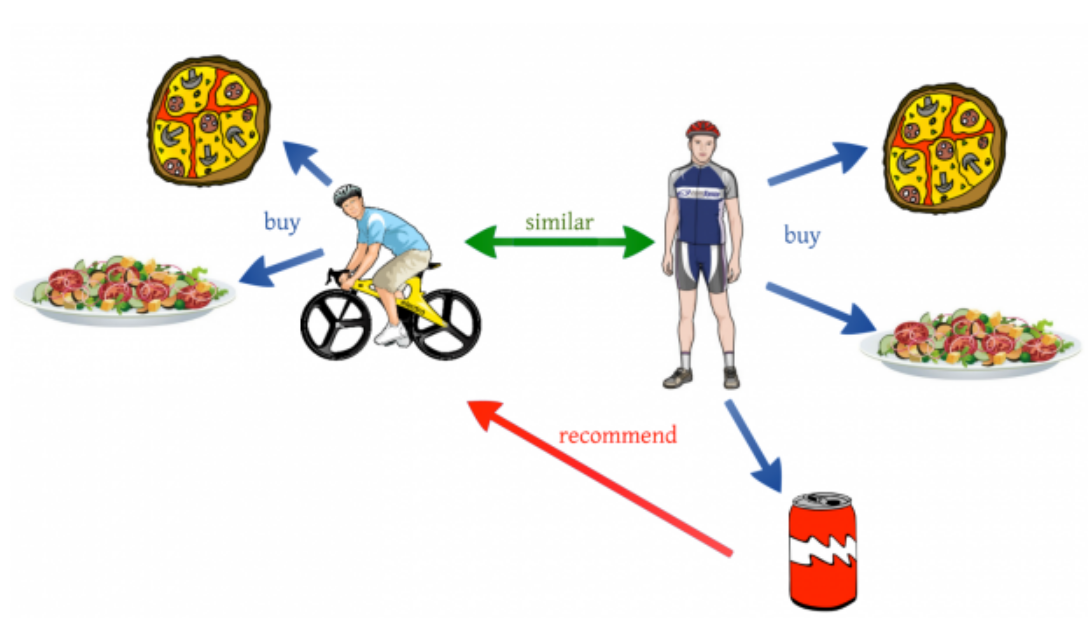
\includegraphics[width=0.6\textwidth]{images/collaborative_filtering.PNG}
    \caption{Illustration of Collaborative Filtering}Credit:\href{https://towardsdatascience.com/various-implementations-of-collaborative-filtering-100385c6dfe0}{here}
    \label{fig:collaborative_filtering}
\end{figure}
By combining insights from both association analysis and customer buying behavior, we tailored product recommendations to individual customers. To prioritize recommendations, we used customer raking according to their quartile scores.
\begin{figure}[H]
    \centering
    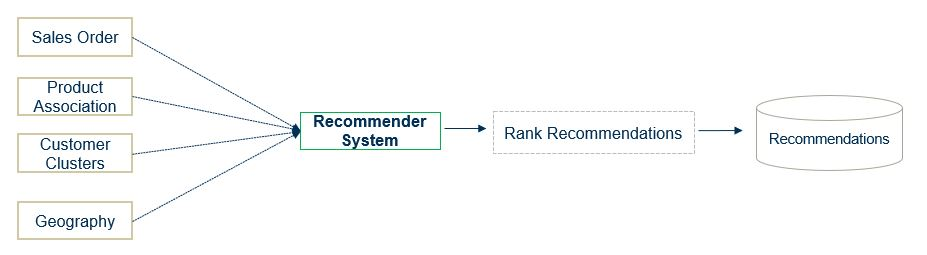
\includegraphics[scale=0.7]{images/customer_recommendation_methods.JPG}
    \caption{Customer Recommendation Process Flow}
    \label{fig:customer_recommendation_methods}
\end{figure}
\clearpage
\section{Analysis and Results}
In order to perform our analysis, we used python, seaborn package for EDA, mlxtend package\cite{12}\cite{13} for association rule mining and built the logic in python for implementing collaborative filtering.
\textbf{Which products are associated and can be bundled together for up-sell and cross-sell?}\\\\
In order to identify the products those are closely associated with another product, we perform association rule mining and get all possible combinations thru customer invoice purchase and filtered the association where confidence is greater than 50\% and Lift is greater than 10.Below products are strongly associated and can be bundled together for upsell \& cross sell. 
\begin{table}[H]
\small
\begin{tabular}{@{}lp{4cm}p{4cm}lll@{}}
\toprule
\multicolumn{1}{c}{\textbf{\begin{tabular}[c]{@{}c@{}}Association\\ Rule\end{tabular}}} & \multicolumn{1}{c}{\textbf{\begin{tabular}[c]{@{}c@{}}Focus \\ Product\end{tabular}}} & \multicolumn{1}{c}{\textbf{\begin{tabular}[c]{@{}c@{}}Associated \\ Product\end{tabular}}} & \multicolumn{1}{c}{\textbf{Confidence}} & \multicolumn{1}{c}{\textbf{Lift}} & \multicolumn{1}{c}{\textbf{Support}} \\ \midrule
1                                                                                       & \#10 White Business Envelopes,4 1/8 x 9 1/2                                           & Staples                                                                                    & 100\%                                   & 27.78                             & 0.001241                             \\
2                                                                                       & Microsoft Natural Ergonomic Keyboard 4000                                             & Boston 16765 Mini Stand Up Battery                                                         & 67\%                                    & 537.00                            & 0.001241                             \\
3                                                                                       & Great White Multi-Use Recycled Paper (20Lb. and 84 Bright)                            & Advantus Rolling Storage Box                                                               & 67\%                                    & 214.80                            & 0.001241                             \\
4                                                                                       & GBC Wire Binding Combs                                                                & Carina Double Wide Media Storage Towers in Natural \& Black                                & 67\%                                    & 179.00                            & 0.001241                             \\
5                                                                                       & O'Sullivan 4-Shelf Bookcase in Odessa Pine                                            & GBC Standard Recycled Report Covers, Clear Plastic Sheets                                  & 50\%                                    & 201.38                            & 0.001241                             \\
6                                                                                       & Xerox 1894                                                                            & Xerox 225                                                                                  & 50\%                                    & 115.07                            & 0.001241                             \\
7                                                                                       & Tennsco Regal Shelving Units                                                          & Staples                                                                                    & 50\%                                    & 13.89                             & 0.001241                             \\
8                                                                                       & Wirebound Four 2-3/4 x 5 Forms per Page, 400 Sets per Book                            & Staples                                                                                    & 50\%                                    & 13.89                             & 0.001241                             \\ \bottomrule
\end{tabular}
\end{table}
\clearpage
\textbf{Can we create customer segments for bulk recommendations ?}\\
In order to understand the customer purchasing behaviour, we segmented customers using their Recency, Frequency and Monetary values with K-Means clustering and found 5 optimum clusters using the elbow method representing 5 different customer purchase patterns. Further, we studied the purchase pattern using a radar chart which is explained in detail in the table below. For each customer, we created unique recommendation strategy.
\begin{figure}[H]
  \centering
  \begin{subfigure}[b]{0.4\textwidth}
    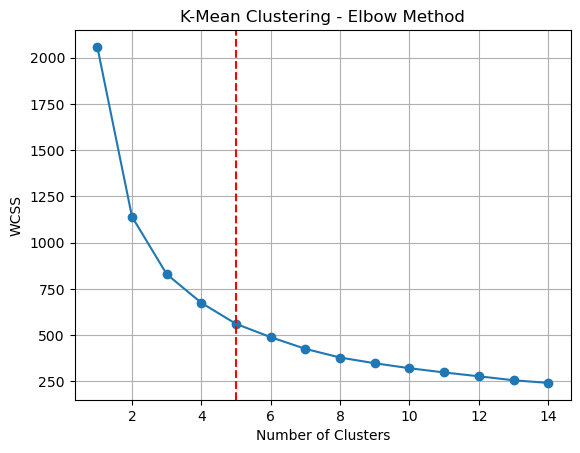
\includegraphics[width=\textwidth]{images/Customer_Clusters.png}
    \caption{Elbow Method to determine Clusters}
    \label{fig:K-Mean Cluster}
  \end{subfigure}
  \hfill
  \begin{subfigure}[b]{0.4\textwidth}
    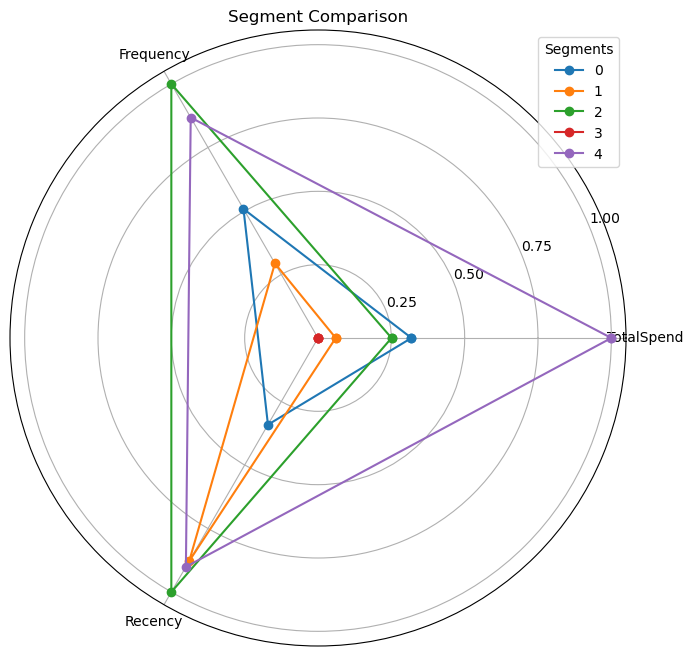
\includegraphics[width=\textwidth]{images/Customer_Clusters_radar.png}
    \caption{Radar chart explaining the clusters}
    \label{fig:Radar Clusters}
  \end{subfigure}
  \caption{Customer Segmentation}
  \label{fig:Customer Segmentation}
\end{figure}
% Table for Product Association
\begin{table}[H]
\small
\begin{tabular}{@{}llllp{4cm}p{4cm}@{}}
\toprule
\textbf{Segment} & \textbf{\begin{tabular}[c]{@{}l@{}}Recency\\(days)\end{tabular}} & \textbf{Frequency} & \textbf{\begin{tabular}[c]{@{}l@{}}Total Spend\\(\$)\end{tabular}} & \textbf{Insights}                                                                                                     & \textbf{Marketing   Strategy}                                                                                                       \\ \midrule
0                & 370.69                                                                  & 6.27               & 2039.29                                                                      & Recent purchasers with high total spend. Likely regular customers   contributing significantly to revenue and profit. & Maintain loyalty with personalized recommendations, special   discounts, and targeted marketing campaigns.                          \\
1                & 853.85                                                                  & 4.5                & 682.61                                                                       & Moderate engagement and expenditure but haven't made recent   purchases.                                              & Re-engage with personalized reminders, limited-time discounts, and   showcasing new products.                                       \\
2                & 963.9                                                                   & 10.32              & 1682.67                                                                      & High frequency of transactions but haven't made recent purchases.   Moderate expenditure.                             & Reactivate with targeted campaigns, personalized messages, and   referral incentives.                                               \\
3                & 63.35                                                                   & 2.08               & 365.14                                                                       & Recent shoppers with moderate engagement and expenditure. Likely new   or occasional shoppers.                        & Implement first-time buyer programs, welcome discounts, and recommend   popular products to increase purchase frequency and amount. \\
4                & 874.46                                                                  & 9.23               & 5620.29                                                                      & Loyal customers with recent purchases, high engagement, and   expenditure.                                            & Strengthen loyalty with exclusive rewards, early access, and feedback   programs.                                                   \\ \bottomrule
\end{tabular}
\end{table}
\clearpage
\textbf{Which customer can be recommended for bundled products ?}\\\\
We adopted Collaborative Filtering method as our recommendation engine and mapped the customers who can be recommended a certain product based on association rule and similar type of customer.We have an overall 15 recommendations. Below are our top 5 recommendations after ranking the recommendations. First column contains the customer to whom we are recommending, second column contains the product we are recommending, third column provides a reference of similar customer product combination who purchased this combination a few times and last column represents the association rule.
% Table Customer Recommendation
% Please add the following required packages to your document preamble:
% \usepackage{booktabs}
% \usepackage[table,xcdraw]{xcolor}
% Beamer presentation requires \usepackage{colortbl} instead of \usepackage[table,xcdraw]{xcolor}
% Please add the following required packages to your document preamble:
% \usepackage{booktabs}
\begin{table}[H]
\small
\centering
\begin{tabular}{@{}lp{3.5cm}p{3.5cm}p{3.5cm}@{}}
\toprule
\multicolumn{1}{c}{\textbf{\begin{tabular}[c]{@{}c@{}}Customer\\ Name\end{tabular}}} & \multicolumn{1}{c}{\textbf{\begin{tabular}[c]{@{}c@{}}Recommended\\ Product\end{tabular}}} & \multicolumn{1}{c}{\textbf{\begin{tabular}[c]{@{}c@{}}Similar Customer - Item \\ Reference\end{tabular}}}                  & \multicolumn{1}{c}{\textbf{\begin{tabular}[c]{@{}c@{}}Recommendation\\ Reason\end{tabular}}}                                         \\ \midrule
JohnLucas                                                                            & Xerox 225                                                                                  & JenniferFerguson:Xerox   1894$\sim$Xerox 225                                                                               & Customer who buys Xerox 1894   also buys Xerox 225                                                                                   \\
FredMcMath                                                                           & Staples                                                                                    & AlanBarnes:Tennsco Regal   Shelving Units$\sim$Staples                                                                     & Customer who buys Tennsco Regal   Shelving Units also buys Staples                                                                   \\
ScottWilliamson                                                                      & Staples                                                                                    & AlanBarnes:Tennsco Regal   Shelving Units$\sim$Staples                                                                     & Customer who buys Tennsco Regal   Shelving Units also buys Staples                                                                   \\
CynthiaDelaney                                                                       & Great White Multi-Use Recycled Paper (20Lb. and 84 Bright)                                 & AlanDominguez:Advantus Rolling   Storage Box$\sim$Great White Multi-Use Recycled Paper (20Lb. and 84 Bright)               & Customer who buys Advantus   Rolling Storage Box also buys Great White Multi-Use Recycled Paper (20Lb. and   84 Bright)              \\
PatrickGardner                                                                       & O'Sullivan 4-Shelf Bookcase in Odessa Pine                                                 & JulianaKrohn:GBC Standard   Recycled Report Covers, Clear Plastic Sheets$\sim$O'Sullivan 4-Shelf Bookcase in   Odessa Pine & Customer who buys GBC Standard   Recycled Report Covers, Clear Plastic Sheets also buys O'Sullivan 4-Shelf   Bookcase in Odessa Pine \\ \bottomrule
\end{tabular}
\end{table}
\clearpage
\textbf{How much revenue opportunity is anticipated ?}\\\\
Customer recommendations value enhances when tied with the business revenue opportunity. Below table depicts high level revenue opportunity for Amazon from the cross-selling \& bundling products to recommended customers.While calculating the revenue opportunity, we considered all 15 customer recommendations, Average Purchase/Year is calculated by taking average qty sold over 2011-2014, Unit Price is calculated dividing Sales Price/Qty, and Opportunity = Unit Price * Average Purchase per Year. We observe a potential opportunity of \$8,000 through these recommendations.
\begin{table}[H]
\small
\centering
\begin{tabular}{@{}lp{4cm}lll@{}}
\toprule
\multicolumn{1}{c}{\textbf{\begin{tabular}[c]{@{}c@{}}Customer   \\ Name\end{tabular}}} & \multicolumn{1}{c}{\textbf{\begin{tabular}[c]{@{}c@{}}Recommended \\ Product\end{tabular}}} & \multicolumn{1}{c}{\textbf{\begin{tabular}[c]{@{}c@{}}Unit \\      Price (\$)\end{tabular}}} & \multicolumn{1}{c}{\textbf{\begin{tabular}[c]{@{}c@{}}Avg Qty \\ Sold\end{tabular}}} & \multicolumn{1}{c}{\textbf{\begin{tabular}[c]{@{}c@{}}Opportunity\\ (\$)\end{tabular}}} \\ \midrule
JohnLucas                                                                               & Xerox 225                                                                                   & \$     22.59                                                                                 & 4                                                                                    & \$           83.90                                                                      \\
PenelopeSewall                                                                          & Staples                                                                                     & \$     28.91                                                                                 & 4                                                                                    & \$        104.06                                                                        \\
KalycaMeade                                                                             & Boston 16765 Mini Stand Up Battery Pencil Sharpener                                         & \$     23.32                                                                                 & 2                                                                                    & \$           46.64                                                                      \\
KeithHerrera                                                                            & GBC Standard Recycled Report Covers, Clear Plastic Sheets                                   & \$     20.48                                                                                 & 6                                                                                    & \$        112.65                                                                        \\
FredMcMath                                                                              & Staples                                                                                     & \$     28.91                                                                                 & 4                                                                                    & \$        104.06                                                                        \\
ScottWilliamson                                                                         & Staples                                                                                     & \$     28.91                                                                                 & 4                                                                                    & \$        104.06                                                                        \\
AlanBarnes                                                                              & Carina Double Wide Media Storage Towers in Natural \& Black                                 & \$   310.42                                                                                  & 4                                                                                    & \$     1,189.96                                                                         \\
ChadSievert                                                                             & Staples                                                                                     & \$     28.91                                                                                 & 4                                                                                    & \$        104.06                                                                        \\
CynthiaDelaney                                                                          & Great White Multi-Use Recycled Paper (20Lb. and 84 Bright)                                  & \$     15.07                                                                                 & 3                                                                                    & \$           39.18                                                                      \\
JustinRitter                                                                            & GBC Standard Recycled Report Covers, Clear Plastic Sheets                                   & \$     20.48                                                                                 & 6                                                                                    & \$        112.65                                                                        \\
PatrickGardner                                                                          & O'Sullivan 4-Shelf Bookcase in Odessa Pine                                                  & \$   452.16                                                                                  & 7                                                                                    & \$     2,939.06                                                                         \\
DennyJoy                                                                                & Xerox 225                                                                                   & \$     22.59                                                                                 & 4                                                                                    & \$           83.90                                                                      \\
MarkHaberlin                                                                            & O'Sullivan 4-Shelf Bookcase in Odessa Pine                                                  & \$   452.16                                                                                  & 7                                                                                    & \$     2,939.06                                                                         \\
\textbf{Total}                                                                          & \textbf{}                                                                                   & \textbf{}                                                                                    & \textbf{}                                                                            & \textbf{\$     7,963.23}                                                                \\ \bottomrule
\end{tabular}
\end{table}
\section{Conclusions}
In our research, we analyzed the Amazon sales dataset obtained from Kaggle, covering sales data spanning the period from 2011 to 2014. We examied the sales data and uncovered notable product associations, such as Wirebound Four 2-3/4 x 5 Forms per Page, 400 Sets per Book, and Staples, Xerox 1894 \& Xerox 225, among others. This discovery underscored the potential for bundled product offerings and informed our subsequent strategies. We proceeded to segment customers based on Recency, Frequency, and Monetary (RFM) values, leading to the identification of five distinct customer groups. These groups included customers characterized by recent purchases and high spending, moderate engagement and spending, high frequency and moderate expenditure, as well as those exhibiting recent purchases with moderate expenditure and high frequency. Subsequently, we tailored targeted selling strategies tailored to each group's specific characteristics. Leveraging insights from product-customer combinations, we formulated personalized recommendations for customers, enhancing their shopping experience and satisfaction. Finally, through comprehensive analysis, we quantified the up-sell and cross-sell revenue opportunities resulting from our marketing efforts, revealing a potential gain of \$8,000 from with just a few strategic combinations. These findings underscore the effectiveness of our approach in optimizing sales and maximizing revenue opportunities within the Amazon ecosystem.
\section{Lesson Learned}
Performing thorough analysis of the Amazon sales dataset, several key lessons emerged. Firstly, we didn't have enough orders with repetitive purchase combination to straighten our association rules. We need more data to solidify are recommendations. Secondly, the segmentation of customers based on Recency, Frequency, and Monetary (RFM) values provided valuable insights into customer behavior, we would liked to have customer profiling information like age-group, gender and geography to tighten our marketing approach.
Subsequently, due to lack of above information, we were not able to experiment with hybrid recommender system which is a combination of content \& collaborative filtering.
Lastly, we were not able to compare our results with ground truth for cross-validation.In real world scenarios, we sit with sales and marketing team to validate the associations.
\section{Future Improvements}
Exploring larger datasets presents an opportunity to unearth even more lucrative product combinations, thereby enhancing our ability to maximize revenue potential. Additionally, developing an application dedicated to recommendations, coupled with soliciting and incorporating customer feedback, can significantly enhance the efficacy of our recommendation engine, ensuring it remains relevant and valuable to users. Furthermore, integrating hybrid recommender methodology into our recommendation system can further refine and improve the accuracy of our recommendations, enriching the customer experience and fostering increased engagement with our platform.

\section{Bibliography and Credits}
% Your bibliography section
\begin{thebibliography}{5}

    \bibitem{1}
    {anandshaw2001}
    anandshaw2001. (2024, March 4). \textit{Amazon\_Sales\_Dataset}. Kaggle. \url{https://www.kaggle.com/datasets/anandshaw2001/amazon-sales-dataset?resource=download}
    
    \bibitem{2}
    Amazon selling stats - sell on Amazon. (n.d.). https://sell.amazon.com/blog/amazon-stats 
    
    \bibitem{3}
    M. Saranya. (2023, July 25). \textit{Amazon sales analysis}. LinkedIn. \url{https://www.linkedin.com/pulse/amazon-sales-analysis-saranya-m/}
    
    
    \bibitem{4}
    According to the analysis conducted by J. Miglani (2023), titled \textit{Amazon Sales and Profit Analysis for 2022: Top 10 Insights}, which was posted on Forrester's blog, the analysis can be accessed through the following link: \url{https://www.forrester.com/blogs/amazon-sales-and-profit-analysis-for-2022-top-10-insights/}.
    
    
    \bibitem{5}
    Vamanan, Dilip. (2024, February 16). \textit{How to grow your profits with Amazon Data Analytics}. SellerApp Blog. \url{https://www.sellerapp.com/blog/amazon-data-analytics/}

    \bibitem{6}
    Saji, B. (2024, January 7). \textit{Elbow method for finding the optimal number of clusters in K-means. Analytics Vidhya}. \url{
    https://www.analyticsvidhya.com/blog/2021/01/in-depth-intuition-of-k-means-clustering-algorithm-in-machine-learning/}

    \bibitem{7}
    “51 Customer Service Statistics You Need to Know.” Zendesk, 13 Feb. 2024, \url{www.zendesk.com/blog/customer-service-statistics/}.

    \bibitem{8}
    Bedgood, Larisa. “69\% of Companies Say Personalized Experiences a Priority.” Porchgroupmedia.com, 2017, \url{https://porchgroupmedia.com/blog/69-companies-rate-personalizing-customer-experience-top-priority}.

    \bibitem{9}
    “(PDF) Explaining Customer Ratings and Recommendations by Combining Qualitative and Quantitative User Generated Contents.” ResearchGate, \url{www.researchgate.net/publication/331337561_Explaining_customer_ratings_and_recommendations_by_combining_qualitative_and_quantitative_user_generated_contents}.

    \bibitem{10}
    Chatterjee, Dr. Swagato. “Explaining Customer Ratings and Recommendations by Combining Qualitative and Quantitative User Generated Contents.” Decision Support Systems, vol. 119, Apr. 2019, pp. 14–22, \url{www.sciencedirect.com/science/article/pii/S0167923619300363, https://doi.org/10.1016/j.dss.2019.02.008}.

    \bibitem{11}
    Roy, Deepjyoti, and Mala Dutta. “A Systematic Review and Research Perspective on Recommender Systems.” Journal of Big Data, vol. 9, no. 1, 3 May 2022, \url{https://doi.org/10.1186/s40537-022-00592-5}.

    \bibitem{12}
    Raschka, Sebastian. “Association Rules - Mlxtend.” Rasbt.github.io, \url{rasbt.github.io/mlxtend/user_guide/frequent_patterns/association_rules/}.

    \bibitem{13}
    ---. “Mlxtend: Machine Learning Library Extensions.” PyPI, \url{pypi.org/project/mlxtend/}.

\end{thebibliography}

\end{document}
